\section{Introduction}
In scientific research \cite{}, software engineering and cybersecurity \cite{}, politics \cite{}, and daily life \cite{}, individuals face problems that involve many interdependent variables and thus large problem spaces, although only sparse -- or unique -- solutions exist \cite{}. These problems are known to be hard to humans, and have been studied by cognitive scientists \cite{Neurath's boat}. In cognitive science, reverse-engineering a Bayesian Network, which involves complicated interdependencies, has become a typical way to probe cognitive capabilities \cite{}. Because variables are dependent, landscapes are not smooth and solutions cannot be reached by simple local search/optimisation strategies {\bf (could we illustrate this point in a way or another with a figure?)}. 

Here, we investigate the fine-grained cognitive mechanisms of complicated problem resolution, which involves 2 treatments {\bf for} the resolution of 3-node and 4-node Bayesian networks over one trial of XX minutes, with a warm-up period of YY. Reverse-engineering these Bayesian networks involve evaluating respectively 8 and 16 conditional probabilities (varying from $0$ to $1$). Any change to any of these probabilities is registered with a resolution of one second [see Supplementary Information (SI) \ref{SI_experiment}]. On average, participants perform poorly in both treatments (see Figure \ref{fig:1}A), and improvement of the proposed models over time follows an extremely slow decay [with Jensen-Shannon Distance $D_{jsd}(t) \sim t^{\nu}$ with $ \nu \approx -0.15(1)$]. 

\begin{figure}[h!]
\begin{center}
\includegraphics[width=17cm]{figures/figure1.eps}
\caption{\footnotesize{{\bf A.} Average Euclidian Distance $\langle D \rangle$ decays as function of time as $\sim t^{\nu}$ with $ \nu \approx -0.15(1)$ indicating a very slow convergence to the true model {\bf [indicate $t_0$s and what their values may mean]}. {\bf B.} Probability density function of displacement $pdf(\Delta r) = \Delta r^{-\alpha -1}$ with $\alpha = 0.40(5)$ with a cut-off limited by the largest possible displacement, which is $\sqrt{k}$ with $k$ the number of conditional probabilities to evaluate. {\bf C.}  Probability density function of waiting time $\Delta t$ $pdf(\Delta t) = \Delta t^{-\beta -1}$ with 2 regimes : $\beta_{\Delta t < 125} = 0.38(4)$ and $\beta_{\Delta t > 125} = 1.59(5)$. Distributions of $\Delta r$ and $\Delta t$ are equivalent for the simple and complex treatments.}}
\label{fig:1}
\end{center}
\end{figure}

Humans -- like many other animals \cite{} -- use efficient strategies to search for food over large areas \cite{rhodes2007human}. These L\'evy walks strategies alternate many small local displacements and few long range displacement. Namely, the distribution of displacements obeys a power law: 

\begin{equation}
\label{displacements}
pdf(\Delta r) = \Delta r^{-\alpha -1}.
\end{equation}

We find that displacements between proposed models (on average over all participants) follow a similar power law distribution with $\alpha = 0.40(5)$ (see Figure \ref{fig:1}B). In addition, the distribution of waiting times $\Delta t$ between two iterations of model propositions, also follows a power law: 

\begin{equation}
\label{wtimes}
pdf(\Delta t) = \Delta t^{-\beta -1},
\end{equation}

with 2 regimes : $\beta_{\Delta t < 125} = 0.38(4)$ and $\beta_{\Delta t > 125} = 1.59(5)$. Distributions of $\Delta r$ and $\Delta t$ are equivalent for the simple and complex treatments. Together, equations \ref{displacements} and \ref{wtimes} define a Continuous Time Random Walk (CTRW) \cite{}, which is another flavour of food search for {\bf XXXanimals} in ecological systems \cite{book_ecological_systems}. The observed displacement exponent is significantly smaller, compared to optimal L\'evy walks of food search in ecosystems, typically found close to  $\alpha = 1$ \cite{} and mathematically optimal for search of sparse solutions in wide areas, provided that search is a memoryless process \cite{viswanathan1999optimizing, edwards2007revisiting,song2010modelling,viswanathan2011physics}. \\

\subsection{Memory in L\'evy Walks/Flights}

However, humans exhibit repeated behaviours, which imply memory. For instance, evidence from online auctions \cite{radicchi2012rationality}  suggests that optimal search strategy ($\alpha = 2 $) can be reached by humans when considering evolutionary forces \cite{radicchi2012evolution}. Sedentary human mobility (e.g., in cities) also exhibits repeated travel behaviours, such as between home and work places, with short displacements around few areas of particular interests, and with punctual travels beyond the borders of the city, e.g., to another city or country \cite{brockmann2006scaling,gonzalez2008understanding,song2010modelling}. Using mobile phone traces, Song et al.  have proposed a modified version of L\'evy flights, by incorporating a form of preferential attachment, which predicts that most visited places tend get even more visits \footnote{The model proposed by Song et al. \cite{song2010modelling} is however a challenge to common sense logic: Most visited places (i.e., home and workplace) are visited at a stable rate, roughly following circadian periods.}. Yet, on the contrary to early models \cite{viswanathan1999optimizing, edwards2007revisiting,song2010modelling,viswanathan2011physics}, proposed explanations by Radicchi et al. \cite{radicchi2012evolution} and Song et al. \cite{song2010modelling} incorporate memory, either through evolutionary forces to optimise online auction strategies (through {\it try and fails}), or human memory driving routine repeated visits of same places \cite{gonzalez2008understanding,song2010modelling}, because they bring renewal resources (mainly financial resources are derived from staying at work, while home may bring e.g., a roof for the night, rest and intrinsic rewards). {\bf Although we have not found documented evidence of memory for animals and nomad humans (such as e.g., hunter gatherers), they may similarly perform L\'evy flights with memory, returning to previously visited food spots, which have replenished between two visits [$\rightarrow$ is there a chance to find evidence for this, even if it's qualitative? I am really surprised this has not been documented yet.]}.\\

%\ref{fig:3}A ???


\subsection{An experiment to probe cognitive mechanisms involved for solving hard problems}

Hard problems {\bf [provide a strict definition of hard problems above, as much as possible, or refine terminology]} have a unique best solution, which can be approached. yet getting close to this solution is hard, because many interdependent variables are involved. 

Individuals tackling hard problems face a tension between testing and updating their beliefs from information stored in their memory (i.e., {\it exploitation} or {\it recombination of information}), and taking action to {\it explore} and update their belief from not previously available {\it exogenous} information. Taking such action would equivalent to the exploration of unknown territories by pioneers in the physical world. The former {\it exploitation} approach may bring improvement toward the solution, however limited to a {\bf (linear?) combination} of previously tried solutions. The latter approach is a {\bf more} high-risk high-return strategy, but whether it brings improvement towards the solution or not, it matters little, as this strategy primarily expands the {\bf convex hull of the explored portion of the solution space [not sure if we can say it this way]}. Once a new portion of the solution space has been explored, the attempted proposed model is then stored into memory and may be recombined, later on, with other proposed models. \\
\begin{figure}[h!]
\begin{center}
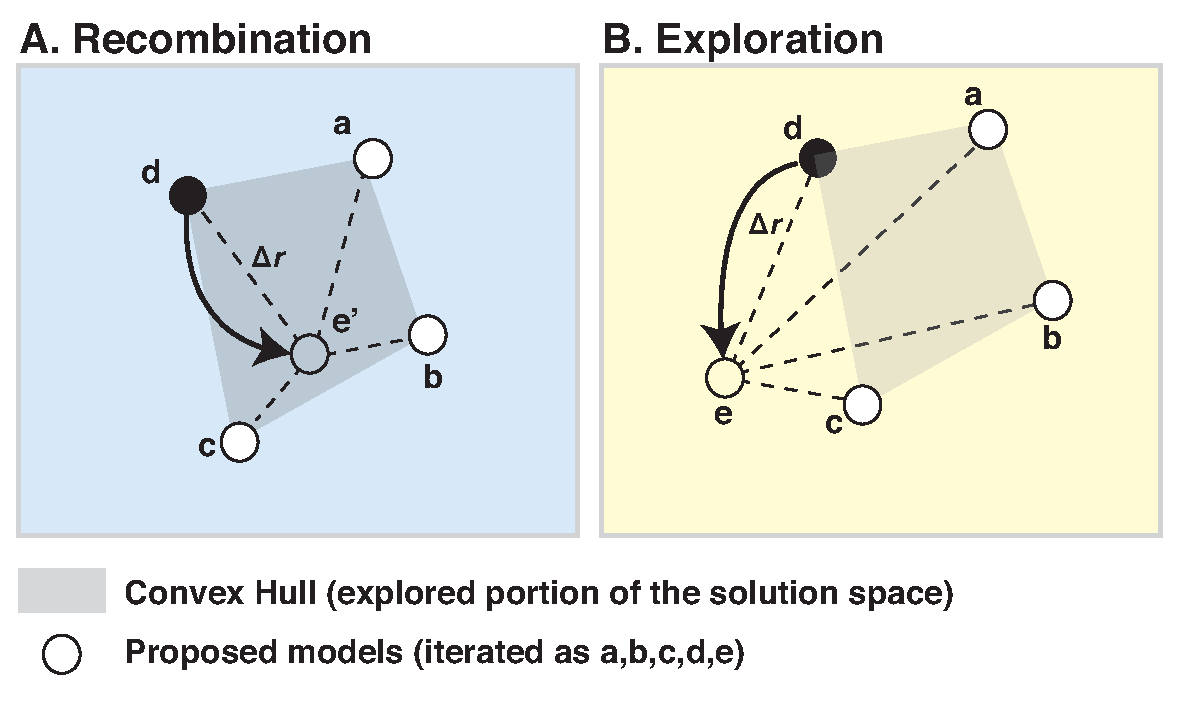
\includegraphics[width=12cm]{figures/figure2.eps}
\caption{\footnotesize{Simplified diagram of exploration and recombination on a plane: {\bf A. Recombination:} iteration {\bf e'} does not incorporate new information. It is a {\bf (linear?)} combination of all previous proposed solutions (i.e., $\{a,b,c,d\}$).  {\bf B. Exploration:} the average distance between iteration {\bf e} and all previous iterations is larger than half of the maximum distance between any previous proposed solutions. Exploration is not memoryless: {\bf e} is closer to {\bf c} and {\bf d} than {\bf a} and {\bf b}. }}
\label{fig:2}
\end{center}
\end{figure}

There is a dearth of knowledge on how the exploration out of the convex hull brings new information, which is then recombined with previously acquired knowledge, stored in memory (see Figure \ref{fig:2}A). Exploration is not memoryless and still occurs by leveraging memory (see Figure \ref{fig:2}B). While exploration entails a pure luck component (beyond the previously explored convex hull), recombination could be optimised to find the best possible recombination, which corresponds to the optimal proposed solution (i.e., as close as possible from the true solution) within the currently explored convex hull.\\

The experiment conducted at Columbia University Social Science laboratory with 96 participants asked to reverse engineer a Bayesian Network with its conditional probabilities and dependencies between nodes show the very fine grained mechanisms of how people struggle balancing recombination of information stored in memory and exploration beyond the currently known convex hull as a subset of the solution space. Our results suggest that displacement $0.1 < \Delta r < 0.2 $ is particularly beneficial for making progress toward the correct solution. We also find that large displacements orders of magnitude more ``brain processing" time compared to small displacements {\bf [how can we make sure that this is truly brain processing time and not an artefact from the web interface?]}. Displacement $0.1 < \Delta r < 0.2 $ is precisely at the inflexion point before waiting times get punishingly long. Yet it remains unclear if some participants manage to consistently use this {\bf ``best strategy"} or if performance is mainly a matter of luck.


This article is organized as follows. We first report on the experimental results, in particular deviations from a memoryless L\'evy Walks/Flights, such as peculiar returns to previously visited solutions, {\bf anomalous mean square displacement following return and recombination [more work is needed here]}, explorations beyond the convex hull, as well as waiting-time and long-memory processes. We then show memory, exploration and recombination influence performance. {\bf Building on theoretical consideration in conjunction with observed stylized facts, we test a model of mechanics of cognition when people tackle hard problems [remains to be done. It may incorporate some Hawkes Processes, but not 100\% sure yet]}. 



\clearpage

%The cognitive  as well as the evolutionary \cite{radicchi2012evolution} underpinnings of L\'evy walks by humans has been questioned and investigated. The ramifications of L\'evy walks in the mind with foraging / mobility patterns in the physical space: here we question if 
%our mind has been shaped by evolutionary pressure and humans resort to similar strategies. Recent research on online bids \cite{radicchi2012rationality} found similar L\'evy walk patterns even though they appear sup-optimal and even slightly irrational, hence suggesting that L\'evy walks are somehow hard coded in our mind  \cite{radicchi2012evolution}, as humans resort to search strategies, which are no longer fit in the world of information and reasoning with abstract problems, which resolution brings its own incentives and resource rewards in the form of money, recognition, reputation, and pleasure \cite{rewards_modern_societies}.\\

%Here, considering humans facing a hard problem -- typically a unique solution in a complicated problem space -- mental search patterns may be inherited from similar L\'evy walks/flights foraging and mobility patterns �\cite{rhodes2007human,radicchi2012rationality,radicchi2012evolution}.\\

%However, these findings were based on specific cases, involving a specific type of auctions \cite{baronchelli2013levy}. It is also considered that the strategy used is L\'evy walks/flights because it is optimal. However, only truly random L\'evy walks/flights are optimal. True randomness is equivalent to a memoryless process, which would allow exploring the solution space with no consideration of previous knowledge. (a evolutionary theory framework is used to rationalise their findings).\\

%Searching for (or tending/optimizing to) a unique solution involves try and fail, and progressive learning. One may think of an evolutionary process (e.g., ``Animals explore the environment mainly for searching food resources, and it is therefore plausible to ascribe the optimality of their search strategies to a selective evolutionary process."  \cite{radicchi2012evolution}), a Markov process \cite{}, or a process with long range memory, in which candidate solutions explored in the past are reused, and recombined with more recent explored solutions. Finally, some new solutions are truly explored out of the currently explored solution envelop.\\
 
% \subsection{Experiment}
%In our experiment, participants were asked to reverse engineer a Bayesian network. They were given 40 minutes, and all changes made were recorded at a 1 second resolution. Participants trying to reverse the best solution face a though problem: The {\it simple} Bayesian network has 3 nodes, and is defined by a 8-parameters vector $\mathbf{s}$ with $0 \leqslant s_k  \leqslant 1$ for $k = \{1,...,8\}$ (resp. $k = \{1,..., 16\}$ for the 4 node {\it complex} Bayesian network). 
 
 
%\subsection{L\'evy Flight / CTRW}
%We first find that the search process follows a L\'evy flight process with waiting times between moves are random variables, which can be accounted together as a continuous time random walk. Both the distributions of displacement (Figure \ref{fig:pdfs}A ) and waiting times (Figure \ref{fig:pdfs}B ) exhibit power law distributions  (Probability density function of displacement $pdf(\Delta r) = \Delta r^{-\alpha -1}$ with $\alpha = 0.40(5)$. {\bf B.} Probability density function of waiting time $\Delta t$ $pdf(\Delta t) = \Delta t^{-\beta -1}$ with 2 regimes : $\beta_{\Delta t < 125} = 0.38(4)$ and $\beta_{\Delta t > 125} = 1.59(5)$. Distributions of $\Delta r$ and $\Delta t$ are equivalent for the simple and complex treatments.){\bf Problem :} Such CTRW process should normally follow ballistic diffusion characterized by mean square displacement (MSD) and diffusion $\sim t^{\mu}$ with  $\mu_{Levy} = 1$ or super-diffusion $\mu_{CTRW} = \beta$ \cite{21,23}). Here, however, mean square displacement (MSD) decays as $\sim t^{\mu}$ with $\mu_{simple} =-0.23(2)$ and $\mu_{complex} =- 0.26(1)$ showing a slow convergence. 

 
 %Here, we document how such frustrating and somewhat irrational situations may stem from evolutionary homology \cite{evolutionary_homology}, that is mental search properties may share conserved neural substrates with similar neuro-molecular processes guiding spatial search in animals and modulating the control of human attention \cite{hills2006animal}. We show that search strategies inherited from food \cite{food_foraging} and resource \cite{resource_foraging} foraging lead to a form of ``hard-wired bounded rationality" when tackling hard problems.\\

%This behavior is at odds with L\'evy walks food search strategies 
%\cite{iswanathan2011physics} used by number of animals 
%\cite{viswanathan1996levy,reynolds2007displaced,edwards2007revisiting,ramos2004levy} and hunter gatherers 
%\cite{brown2007levy}. L\'evy walks which displacement obeys a power law distribution 
%$P(R > \Delta r) \sim \Delta r^{\alpha}$ with $ 0 < \alpha \leqslant 2 $ are known maximize 
%displacement through a super-diffusive process, while minimizing the probability to return to an 
%already visited site (on the contrary to Brownian motion \cite{humphries2010environmental,mendez2013stochastic}). In 
%particular, the food search process in nature has also been found to be optimal $\alpha \approx 1$ 
%\cite{viswanathan1999optimizing}, in the case of Hadza hunter-gatherers in Tanzania 
%\cite{raichlen2014evidence}, and for the dissemination of mussels \cite{de2011levy}. In the latter 
%case, the optimal search process stems from the cooperative organization of mussels, and how 
%this cooperation shapes the environment \cite{de2011levy}. Human mobility traced by banknote circulation \cite{brockmann2006scaling} or mobile phone tracking \cite{song2010modelling,rhee2011levy} also exhibits highly regular L\'evy walk patterns \cite{gonzalez2008understanding}.

%There is suggestive evidence that some cognitive mechanisms, such as information/memory retrieval follows a L\'evy walk \cite{hills2012optimal} with some limited analogy with optimal foraging \cite{rhodes2007human} {\bf (in \cite{rhodes2007human}, it's unclear why the waiting times should be optimal with $\mu \rightarrow 1$. The optimality is in space, optimality is less clear in time)}. {\bf (random walks \cite{abbott2015random})}

%For some time now, cognitive scientists have posed that modeling people's beliefs about causation in the material world provides an effective explanatory framework for how we process information and learn from these observations \cite{Griffiths2008}.  Probabilistic causes and effects, in other words, make up an important construct we seem to make use of when we seek to understand our world.  Bayes Nets are well-defined mathematical objects corresponding to an intuitive representation of causal beliefs.  They are easy to manipulate, do inference with and use as a means to compare different beliefs.  The kinds of Bayes Nets that have been allowed for in experimental settings up to this point, however, have been extremely simplistic and there has been an unanswered call for learning experiments with increased complexity (Griffiths?).  Our work is to our knowledge the first answer to this call.

%From financial stability to the stability of democracies, beliefs play a central role in our explanation of many phenomena. In the social sciences, these beliefs are often conceptualized as probabilistic assessments over states of the world.  However, they are derived from coherent belief systems people hold in their minds regarding how the world works as supported by recent work in cognitive science \cite{lombrozo2006structure, anderson1990cognitive}.  How do humans learn in simple and in complex systems?  How efficiently do they explore the space of possible beliefs and how closely is the direction of exploration tied to experience?  Bayesian approaches of learning would not be feasible for learning in realistically complex systems, given recall constraints and they are not defined in cases where initial beliefs are such that they put zero weight on some possible outcomes.

%Our work presents new experimental results on the rate at which people learn in more or less complex environments. We find that learning rates are much slower than they would be if learners were Bayesians, as had been proposed in older economic theories \cite{Boyer84, Prescott72, Rothschild74, McLennan84, Mirman84, Easley89, Kiefer89}. We also find that the learning rate is slightly higher when people build models of systems that are less complex and that even if the rates were identical accross levels of complexity, accuracy is always higher when the system is structurally simpler because initial models are closer aligned with reality.

%When searching for solutions to outstanding problems, in this case the formation of coherant belief structures that explain experience, humans must come up with innovative solutions.  We show that their strategies look a lot like a class of random search processes in which complete random guessing is strategically combined with the consolidation of past and current experience. We show how people shape their beliefs, starting with complete guesswork through a process that can be accurately modeled as a L'evy random search process, which involves both synthesis of current knowledge (mental exploitation) and out-of-the box mental exploration (see Figure \ref{fig:schematic}). Such random search processes are ubiquitous across the life sciences, in cognitive science, computer science  and artificial intelligence. We then measure how this process leads to convergence, albeit slow, to the correct stochastic solution.

%As can be seen in Figure \ref{fig:decay}, the distance between a person's evolving belief system about some physical system and the long-run absorbing distribution, which we interpret as a performance score, decays with time in a very specific way:
%
%\begin{equation}
%\label{ }
%d(belief_{i, t}, absorbing distribution) = \alpha*t^{-\beta_i}
%\end{equation}
%
%The functional form of human learning in the context of our experiment, then, is the same as for the Bayesian learner, but the decay rate, $\beta$, of a human learner is much smaller than that of a Bayesian.
